\documentclass[paper=a4,fontsize=12pt]{scrartcl}
\usepackage[utf8]{inputenc}
\usepackage[ngerman]{babel}
\usepackage[babel, german=quotes]{csquotes}
%\usepackage[hidelinks]{hyperref}
\usepackage[style=authoryear, natbib]{biblatex}
\usepackage[margin = 2.5cm]{geometry}
\usepackage{graphicx, fancyhdr, array, wrapfig, colortbl, algorithm, algpseudocode}
\floatname{algorithm}{Algorithmus}
\renewcommand{\listalgorithmname}{Algorithmenverzeichnis}
\renewcommand{\algorithmicend}{\textbf{Ende}}
\renewcommand{\algorithmicif}{\textbf{Falls}}
\renewcommand{\algorithmicthen}{\textbf{dann}}
\renewcommand{\algorithmicelse}{\textbf{Sonst}}
\renewcommand{\algorithmicdo}{\textbf{}}
\renewcommand{\algorithmicwhile}{\textbf{Solange}}
\renewcommand{\algorithmicreturn}{\textbf{Returniere}}
\renewcommand\familydefault{\sfdefault}
\linespread{1.5}
\setlength{\parindent}{2mm}
\setlength{\parskip}{2mm}
\pagestyle{fancy}
\fancyhf{}
\clubpenalty = 10000
\widowpenalty = 10000 \displaywidowpenalty = 10000
\fancyfoot{}
\rfoot{{\footnotesize \textnormal{\thepage}}}
\rhead{{\footnotesize \textnormal{}}}
\cfoot{{\footnotesize \textnormal{Lorenz Leutgeb, Moritz Wanzenböck}}}
\lhead{{\footnotesize \textnormal{}}}
\lfoot{{\footnotesize \textnormal{\the\year}}}
\begin{document}
% Fügen Sie Ihrer Arbeit einen halbseitigen Abstract an, in dem Sie Forschungsfrage, Zielsetzung, Vorgehensweise sowie die wichtigsten Ergebnisse zusammenfassen.
% Beschreiben Sie in Ihrer Arbeit nicht nur einen Sachverhalt, sondern erarbeiten Sie ein konkretes Projekt und einen praktischen Lösungsansatz.
% Ihre Arbeit muss einen Abstract, ein Literaturverzeichnis, eine Einleitung, einen Hauptteil, ein Resümee und ein Literaturverzeichnis, gegebenenfalls auch ein Abbildungsverzeichnis enthalten.
% Verfolgen Sie einen roten Faden, damit die einzelnen Kapitel Ihrer Arbeit logischer aufeinander aufbauen.
% Belegen Sie Zitate, Quellen und fremdes Gedankengut korrekt.
% https://www.siemens-stiftung.org/fileadmin/user_upload/technisch-naturwissenschaftliche-bildung/schule/schuelerwettbewerb/2013/Tipps_zum_wissenschaftlichen_Arbeiten_2013.pdf
%foobar \cite{Lu2010, Palladino2011, Noronha2006, Li2000, Frota2010, Demange, pcp-instance-page}
\begin{titlepage}
\begin{center}
\vspace*{\fill}
{\Large E}\ {\large I\ N\ R\ E\ I\ C\ H\ U\ N\ G}

\vspace{5mm}

zum

\vspace{5mm}

{\Large\bfseries Schülerwettbewerb 2013}

\vspace{5mm}

der

\vspace{5mm}


\includegraphics{siemens.jpg}

\vspace{5mm}

zum Thema

\vspace{5mm}

{\Huge Variable Neighborhood Search für das Partition Graph Coloring Problem}

\vspace{5mm}

von

\vspace{5mm}

\begin{tabular}{>{\raggedright\arraybackslash}p{.3\textwidth}c>{\raggedleft\arraybackslash}p{.3\textwidth}}
{\large Lorenz Leutgeb} & und & {\large Moritz Wanzenböck} \\
\end{tabular}

\vspace{5mm}

betreut durch

\vspace{5mm}

{\large Dipl.-Ing.\ Dr.\ techn.\ Martin Gruber}

\vspace{5mm}

an der

\vspace{5mm}


\includegraphics[width=5cm]{../img/htl.png}

\vspace*{\fill}
\end{center}
\end{titlepage}
\tableofcontents
\newpage
\begin{abstract}
Betreiber der Internetinfrastruktur stehen vor dem Problem, immer weiter steigende Kommunikationsbedürfnisse befriedigen zu müssen. Dafür müssen entweder die bestehenden Netze effizienter genutzt oder die Infrastruktur erweitert werden.

In dieser Arbeit soll die Kommunikation innerhalb von Glasfasernetzwerken, die Wavelength Division Multiplexing einsetzen, optimiert werden. Damit sollen vorhandene Ressourcen besser ausgelastet und die Anschaffung und der Betrieb neuer Infrastruktur zumindest hinausgezögert werden, womit sowohl Anschaffungs- als auch Betriebskosten eingespart werden können.

Zur Optimierung wird eine Variable Nachbarschaftssuche eingesetzt, eine Metaheuristik, die ausgehend von einer Ausgangslösung diese schrittweise verbessert, bis keine Fortschritte mehr möglich sind. Erste Ergebnisse sind vielversprechend und zeigen das Potenzial dieses Lösungsansatzes.
\end{abstract}

\section{Einleitung}
\subsection{Problemstellung}
Bei der in der Literatur als Partition Graph Coloring Problem bezeichneten Aufgabenstellung handelt es sich um ein Optimierungsproblem aus dem Bereich des Netzwerkdesigns, konkret um die Planung der Kommunikation in Glasfasernetzwerken. In diesen Netzen wird Wavelength Division Multiplexing betrieben, welches es ermöglicht, zwei oder mehr Übertragungskanäle über die selbe Glasfaser zu leiten, wenn jeder Kanal eine andere Wellenlänge verwendet und somit die anderen Übertragungen nicht stört. Um die Komplexität in einzelnen Netzwerkknoten gering zu halten wird davon ausgegangen, dass eine Verbindung von der Quelle bis zum Ziel nur genau eine Wellenlänge nutzt und diese nicht an Knotenpunkten verändert werden kann.

Zwei unterschiedliche Verbindungen können also nur dann über die selbe Netzwerkstrecke transportiert werden, wenn sie verschiedene Wellenlängen verwenden. Weiters ist die maximale Anzahl an möglichen Wellenlängen pro Strecke beschränkt. Minimiert man in diesem Szenario die Anzahl an benötigten Wellenlängen für die gesamten vorab bekannten Kommunikationsbedürfnisse (z.B.\ im großen Maßstab der Datenaustausch zwischen verschiedenen Providern, deren Verbindungen -- solange es zu keinen Ausfällen kommt -- über eine gewisse Zeit als konstant angesehen werden können), schafft man damit Platz für zusätzliche Datentransfers. Damit kann die bestehende Infrastruktur besser ausgenutzt werden, womit Kosten und Energie für den Ausbau und den Betrieb neuer Netzteile eingespart werden können.

Diese Aufgabenstellung kann auf einfache Art und Weise in ein generalisiertes Graph Coloring Problem transformiert werden, bei dem statt einfacher Knoten ganze Cluster von Knoten betrachtet werden müssen: Für jede Kommunikation werden vorab mehrere günstige Wege durch das Netzwerk von der Quelle zum Ziel ausgewählt (z.B.\ auf Basis der Weglänge und/oder der Übertragungsgeschwindigkeit). Jede Kommunikation bildet dabei einen eigenen Cluster, die einzelnen vorselektierten Wege dieser Kommunikation die Knoten innerhalb des Clusters. In diesem Graphen -- in der Folge auch \emph{Konfliktgraph} genannt -- werden zwei Knoten dann miteinander verbunden, wenn die jeweiligen Wege im originalen Glasfasernetzwerk eine gemeinsame Übertragunsstrecke besitzen, sie sich also gegenseitig stören würden, wenn sie die gleiche Wellenlänge verwenden würden (siehe auch Grafik \ref{fig:translation}). Ziel ist es nun, in diesem Graphen für jeden Cluster genau einen Knoten auszuwählen (für eine Kommunikation einen Weg durch das Netzwerk festlegen) und die pro Cluster ausgewählten Knoten so einzufärben, dass keine direkt miteinander verbundenen Knoten die selbe Farbe erhalten (die Farbe entspricht dabei der Zuordnung einer Wellenlänge). Minimiert man hierbei gleichzeitig die Anzahl an benötigten Farben (womit die Grundauslastung des Netzwerks reduziert wird), erhält man das generalisierte (oder auch Partition) Graph Coloring Problem, ein NP-schweres Optimierungsproblem.

\begin{figure}
    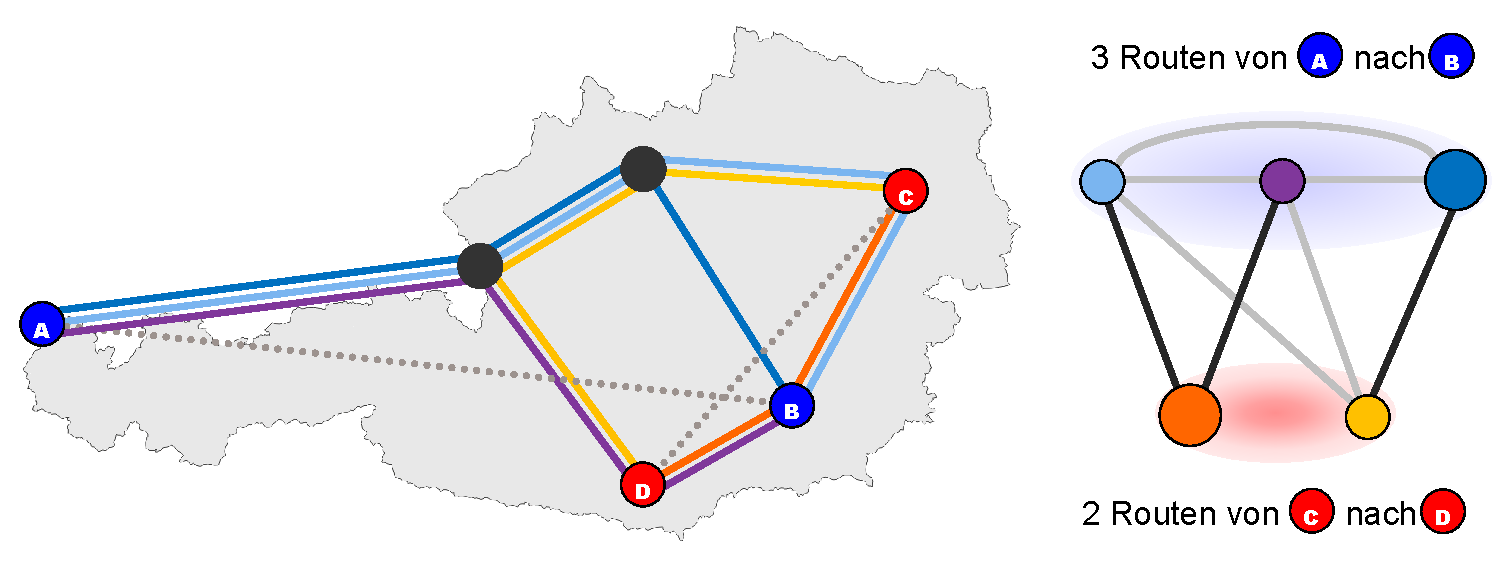
\includegraphics[width=1.0\textwidth]{../img/translation.pdf}
    \caption[Simplifizierte Testinstanz]{Simplifizierte Testinstanz: Für die Kommunikation zwischen \emph{A} und \emph{B} wurden drei mögliche Wege ausgewählt (in Blautönen gehalten), zwischen \emph{C} und \emph{D} zwei Wege (Gelb/Orange). Der daraus resultierende Konfliktgraph auf der rechten Seite enthält zwei Cluster mit drei bzw.\ zwei Knoten und die jeweiligen Kanten, wenn zwei Kommunikationswege zumindest eine Strecke im Netzwerk gemeinsam verwenden. Wählt man die größer dargestellten Knoten innerhalb der Cluster, so kann der Konfliktgraph mit nur einer Farbe gefärbt werden, d.h.\ die Kommunikationsbedürfnisse in diesem Netzwerk können mit nur einer Wellenlänge abgewickelt werden.}
    \label{fig:translation}
\end{figure}

In der Literatur werden exakte Algorithmen beschrieben, die beweisbar optimale Lösungen erzeugen, aber aufgrund der Komplexität des Problems nur auf relativ kleine Netzwerke angewendet werden können. Weiters exitieren einfache Konstruktionsheuristiken für die schnelle Generierung gültiger Ausgangslösungen sowie ein Ansatz mittels Tabu-Suche, der gute Ergebnisse für größere Netzwerke liefert.

\section{Verfahren zur Lösung des generalisierten Graph Coloring Problems}
Im Folgenden sollen bereits bestehende Lösungsansätze für das Partition Graph Coloring Problem vorgestellt und kurz behandelt werden. Außerdem wollen wir unseren eigenen Lösungsansatz vorstellen, welcher auf bereits bestehenden Techniken fußt.

\subsection{Bestehende Lösungsansätze}
Bei unserer Recherche fanden wir bereits einige vorhandene Lösungsansätze für das relativ junge Partition Graph Coloring Problem. \citet*{Li2000} schlugen mehrere Konstruktionsheuristiken vor, welche auch von \citet*{Noronha2006} genutzt wurden, um ihre Tabu-Suche zu implementieren.
Desweiteren gibt es einen Algorithmus von \citet*{Lu2010} sowie einen Ansatz mit Hilfe eines Branch-and-Cut Algorithmus von \citet*{Palladino2011}.

\subsubsection{Konstruktionsheuristiken}
\label{sec:construct}
\citet*{Li2000} beschreiben mehrere schnelle Greedy Algorithmen zur näherungsweisen Lösung des Problems. Im Vergleich der benötigten Farben schneidet dabei der Algorithmus \emph{onestepCD} am besten ab:
\paragraph{onestepCD}{
Zunächst werden in einem Vorverarbeitungsschritt alle Kanten aus dem Konfliktgraphen entfernt, die Knoten innerhalb eines Clusters miteinander verbinden (da für jede Kommunikation nur genau ein Kommunikationsweg gewählt wird, können sich Knoten eines Clusters nie gegenseitig stören, die entsprechenden Kanten sind daher für die Lösung des Problems irrelevant und können gelöscht werden). Danach wird für jeden Cluster der Knoten mit der geringsten Anzahl an bereits eingefärbten Nachbarknoten bestimmt, der Knoten mit der insgesamt kleinsten Anzahl wird ausgewählt. Gibt es hier mehrere gleichwertige Kandidaten, wird aus diesen der Knoten mit der größten Anzahl an noch nicht eingefärbten Nachbarknoten gewählt bzw. -- falls dies immer noch nicht eindeutig möglich ist -- der erste Knoten aus diesen Kandidaten. Nachdem nun ein Knoten als Repräsentant für seinen Cluster bestimmt und ihm die kleinstmögliche Farbe zugewiesen wurde, werden alle anderen Knoten, die sich im selben Cluster befinden, gelöscht. Der Prozess wird solange fortgeführt, bis die Repräsentanten aller Cluster gewählt und eingefärbt sind.
}

Diese Vorgehensweise führt schnell zu einer gültigen Lösung, die aber nur in den seltensten Fällen auch wirklich optimal bezüglich der Anzahl an benötigten Farben ist. Sie kann aber als Ausgangspunkt für Verbesserungsverfahren dienen.
 
\subsubsection{Tabu-Suche}
Mit Hilfe der von \citet*{Noronha2006} vorgeschlagenen Tabu-Suche ist es möglich, eine bereits bestehende Lösung durch verschiedene Transformationen in eine neue, nach Möglichkeit bessere Lösung zu verwandeln.

Zunächst wird bei der Tabu-Suche eine ungültige Lösung erzeugt, und zwar durch das neue Färben aller Knoten, welche in der Ausgangslösung noch die höchste Farbe besaßen, mit einer zufälligen, kleineren Farbe.

Nachdem nun natürlich Konflikte zwischen zwei verbunden Knoten mit der gleichen Farbe entstanden sind, versucht die Tabu-Suche diese Konflikte zu lösen. Dazu wird ein zufälliger im Konflikt stehender Knoten ausgewählt und es wird versucht, diesen neu einzufärben. Sollte dies Erfolg haben beginnt die Tabu-Suche wieder bei der Suche nach in Konflikt stehenden Knoten.

Sollte für einen Knoten allerdings keine passende Farbe gefunden werden können, wird dieser Knoten auf die Tabu-Liste gesetzt, wo er für einige Iterationen verbleibt. Knoten sind, solange sie auf dieser Liste sind, tabu für eine Neueinfärbung, dürfen also nicht ausgewählt werden.

Ist die Tabu-Suche nun nach mehreren Iterationen zu einer validen Lösung gekommen, welche weniger Farben als die Ausgangslösung verwendet, wird sie erneut aufgerufen, um nach Möglichkeit wieder ein Ergebnis mit einer Farbe weniger zu berechnen.
Sollte hingegen die Tabu-Suche auch nach vielen Iterationen keine gültige Lösung erzeugen können, bricht sie von selbst ab und gibt ihre Verbesserungsversuche für diese Lösung auf und beginnt mit einer neuen, zufälligen Neufärbung der aktuell besten gefundenen Lösung.

\subsection{Variable Nachbarschaftssuche (VNS)}
Als Ausgangspunkt für unser Projekt setzen wir auf bereits bewährte Techniken aus anderen Bereichen der Optimierung und versuchen, diese bestmöglich für das Partition Graph Coloring Problem einzusetzen.

\subsubsection{Initiallösung}
Um eine gültige Startlösung als Ausgangspunkt der Variablen Nachbarschaftssuche zu berechnen, wird wie gemeinhin üblich eine schnelle Konstruktionsheuristik eingesetzt. Konkret wurde nach der Konsultation von \citet*{Li2000} die dort beschriebene Heuristik \emph{onestepCD} (siehe \ref{sec:construct}) gewählt.

% Im folgenden soll erläutert werden, wie mit diesem Algorithmus eine Lösung gefunden wird.
\subsubsection{Aufbau der Variablen Nachbarschaftssuche}
Bei der Variablen Nachbarschaftssuche handelt es sich um eine metaheuristische Methode, um verschiedenste Optimierungsprobleme zu lösen. Als Metaheuristik bezeichnet man dabei Algorithmen, die andere heuristische (und manchmal auch für Teilprobleme exakte) Optimierungsverfahren steuern und deren Ergebnisse sammeln und kombinieren.

Wie der Name bereits suggeriert versucht eine VNS auf Basis unterschiedlicher Nachbarschaften eine bereits bestehende, nicht optimale Lösung zu verbessern. Eine Nachbarschaft wird im Normalfall durch sogenannte \emph{Moves}, also Züge, definiert, die beschreiben, wie man von einer Lösung zu einer Nachbarlösung kommt, die hoffentlich besser als die Ursprungslösung ist. Ein solcher Zug kann z.B.\ die Auswahl eines anderen Knotens als Repräsentant eines Clusters sein. Kann eine Lösung mit Zügen aus einer Nachbarschaft nicht mehr verbessert werden, dann befindet man sich in einem \emph{lokalen Optimum}, das leider im Normalfall nicht dem globalen Optimum -- der besten möglichen Lösung -- entspricht.

Die Variable Nachbarschaftssuche setzt nun in ihrer Optimierungskomponente (\emph{Variable Neighborhood Descent}, VND) nicht nur eine sondern gleich mehrere unterschiedliche Nachbarschaften hintereinander ein in der Hoffnung, dass ein lokales Optimum einer Nachbarschaft nicht zwangsläufig auch ein lokales Optimum einer anderen Nachbarschaft ist. Man setzt also darauf, dass eine Lösung, die in einer Nachbarschaft nicht mehr verbessert werden kann, in einer anderen Nachbarschaft sehr wohl noch Optimierungspotential besitzt. Diese neue Lösung kann dann vielleicht wieder mit einem Zug aus der ursprünglichen Nachbarschaft verbessert werden und so weiter.

Durchsucht man alle definierten Nachbarschaften systematisch (z.B.\ mittels \emph{Best Improvement} Strategie, d.h.\ von allen möglichen Zügen innerhalb einer Nachbarschaft wird jener gewählt, der die Lösung maximal verbessert) hintereinander und wiederholt nach besseren Lösungen, dann stoppt dieser Prozess erst dann, wenn eine Lösung gefunden wurde, die ein lokales Optimum bezüglich sämtlicher Nachbarschaften darstellt.

\begin{wrapfigure}[11]{r}{0.4\textwidth}
\vspace{-8mm}
\begin{center}
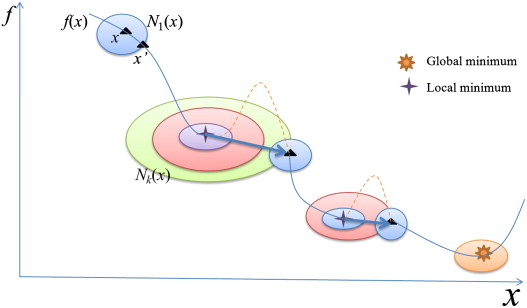
\includegraphics[width=0.4\textwidth]{../img/vns.jpg}
\end{center}
\vspace{-8mm}
\caption{Veranschaulichung der Variablen Nachbarschaftssuche. \cite{Chen}}
\vspace{-8mm}
\end{wrapfigure}

Um diesem Zustand des vollkommenen Stillstandes zu entkommen, wird, nachdem dieses lokale Optimum für alle definierten Nachbarschaften erreicht wurde, mit immer größer werdenden Kraft die Lösung ``geschüttelt''. Gemeint ist damit, dass die lokal optimale Lösung durch verschiedene Algorithmen verändert wird, welche nicht darauf abzielen, eine Lösung besser zu machen, sondern sie zunächst ein wenig, mit dem Fortschreiten der Optimierung aber auch möglichst stark zu verfremden, um einen neuen Startpunkt für das VND zu besitzen.

Veranschaulichen kann man sich das Verfahren, wenn man sich alle gültigen Lösungen als eine große Fläche vorstellt. Je nach Güte der Lösung sind einzelne Teile dieser Fläche unterschiedlich hoch, gute Lösungen bilden Senken (wenige Farben werden für die Färbung benötigt), während schlechte Lösungen Berge bilden. Das VND tendiert nun dazu, sich in einer dieser Senken festzufahren, es wurde ein lokales Optimum bezüglich sämtlicher Nachbarschaften erreicht.

Mit Hilfe des ``Schüttelns'' wird nun versucht, aus eben jenen Senken zu entkommen, um eine andere, hoffentlich tiefere Senke zu finden, also eine bessere Lösung. Nach diesem Schritt beginnt der Algorithmus nämlich wieder von vorne und sucht mit Hilfe der Nachbarschaften erneut ein lokales Optimum.

Obwohl die Variable Nachbarschaftssuche in der Theorie immer weiter laufen könnte und dabei hoffentlich immer wieder neue, bessere Lösungen erreicht, wird meist eine fixe Zeit oder eine Anzahl an Iterationen bzw.\ ``Schüttelungen'' ohne Verbesserung als Abbruchkriterium gewählt.

\begin{algorithm}
\begin{algorithmic}[1]
\State Berechne Initiallösung mit \emph{onestepCD}
\While{Terminationsbedingung \textbf{nicht} erfüllt}
\State Führe Variable Neighborhood Descent mit Best Improvement Strategie durch:
\State Nachbarschaft $l \leftarrow 1$
\While{$l \leq 3$ \textbf{und} Zeitlimit nicht erreicht}
\State Führe Nachbarschaft $n_l$ aus
\If {Lösung verbessert \textbf{und} $l\neq 1$} 
\State  $l\leftarrow 1$  
\Else
\State  $l\leftarrow l + 1$
\EndIf
\EndWhile
\If{Beste Lösung verbessert \textbf{oder} $k \geq k_{\mathrm max}$}
\State $k \leftarrow k_{\mathrm start}$ 
\Else
\State $k \leftarrow k + 1$
\EndIf
\State Wähle zufällig Nachbarschaft aus und ``schüttle" Lösung mit $k$ zufälligen Zügen
\EndWhile
\State\Return Beste gefundene Lösung
\end{algorithmic}
\caption{Pseudocode der Variablen Nachbarschaftssuche}
\end{algorithm}

\subsubsection{Nachbarschaften}
\label{sec:neigh}
Wie bereits beschrieben handelt es sich bei Nachbarschaften um einzelne Algorithmen die versuchen, eine gültige Lösung in eine andere, bessere Lösung durch eine relativ kleine Änderung umzuwandeln. Wir haben uns zunächst auf die drei Nachbarschaften \emph{changeColor}, \emph{changeNode} und \emph{DSATUR} konzentiert, wobei weitere Nachbarschaften noch zur Diskussion stehen.

Jede Nachbarschaft bietet auch eine Methode an, eine Lösung zu ``schütteln'', welche ähnlich abläuft wie die Methode zur Suche des jeweiligen lokalen Optimums, allerdings ohne die Beschränkung ausschließlich bessere Ergebnisse zurückliefern zu müssen.

\paragraph{ChangeColor}
Bei dieser sehr einfachen Nachbarschaft, die von der Tabu-Suche aus \citet*{Noronha2006} inspiriert ist, wird versucht, alle Knoten umzufärben, welche mit der höchsten Farbe markiert wurden. 

Um dieses Ziel zu erreichen, werden alle Knoten, welche diese höchste Farbe besitzen, mit einer neuen zufälligen Farbe markiert. Dies führt natürlich unweigerlich zu Konflikten zwischen verbundenen Knoten im Knfliktgraph, d.h.\ zu benachbarten Knoten mit gleicher Farbe. 

Um diese Konflikte zu lösen wird ein zufälliger, im Konflikt stehender Knoten ausgewählt, um ihn mit einer passenden Farbe zu füllen. Zu beachten ist hierbei die Tatsache, das diese passende Farbe kleiner sein muss als die frühere höchste Farbe, da ja eine Verbesserung (eine Reduktion der Farbenanzahl um 1) erzielt werden soll.

Sollte sich keine passende Farbe finden, wird auch dieser im Konflikt stehende Knoten mit einer zufälligen Farbe neu eingefärbt, was im Normalfall zu weitern Konflikten führt. Es wird nun versucht, diesen gesamten Vorgang so lange zu wiederholen bis keine Konflikte mehr bestehen. 

Sollte nach einer gewissen Anzahl an Iterationen keine konfliktfreie Lösung gefunden werden, bricht \emph{ChangeColor} automatisch ab und liefert die letzte valide Lösung zurück.

\paragraph{ChangeNode}
Diese Nachbarschaft baut auf der Tatsache auf, dass man aus einem Cluster nur jeweils einen Knoten auswählen muss. Dazu werden wie bei \emph{ChangeColor} alle Knoten höchster Farbe ausgewählt und umgefärbt.

Nun wird wieder ein zufälliger Knoten aus den entstandenen Konflikten ausgewählt, welcher dann aber durch einen zufälligen Knoten aus dem selben Cluster ersetzt wird. An diesem Knoten wird dann ein neuer Einfärbeversuch unternommen, wobei die maximal zulässige Farbe natürlich wieder kleiner ist als die ursprünglich höchste Farbe.

Dieser Vorgang wird solange wiederholt bis alle Konflikte gelöst wurden oder zu viele Iterationen abgelaufen sind.

\paragraph{NewVertexColoring-DSATUR}
Diese Nachbarschaft reduziert das Graph Partition Coloring Problem auf das normale Graph Coloring Problem ohne Clusterung der Knoten, indem die aktuell gewählten Repräsentanten fixiert werden und dieses so vereinfachte Problem (das allerdings immer noch NP-hart ist) wird nun mit folgendem Greedy Ansatz näherungsweise gelöst:

\begin{enumerate}
    \item Finde den (noch nicht eingefärbten) Repräsentanten mit der größten Anzahl an eingefärbten Nachbarn (engl.\ Degree SATURation).
    \item Bei Gleichstand: Wähle den Knoten mit der größten Anzahl an nicht eingefärbten Nachbarn.
    \item Bei Gleichstand wähle den ersten Knoten in lexikographischer Abfolge.
    \item Weise dem gewählten Knoten die kleinste mögliche Farbe zu.
    \item Wiederhole, bis die Repräsentanten aller Cluster eingefärbt wurden.
\end{enumerate}

\subsection{Implementierung}
Um die im Zuge dieser Arbeit entwickelten Lösungsansätze verifizieren und bewerten zu können, wurde das vorgestellte Konzept (Variable Nachbarschaftssuche mit Ermittlung einer Initiallösung durch \emph{onestepCD}) vollständig implementiert.

Das Programm wurde in C++ entwickelt, da diese Sprache für gute Performance bekannt ist und außerdem etablierte Codebibliotheken, speziell für Probleme der Kombinatorik und Graphentheorie, explizit für C++ zur Verfügung stehen.

Nach einigen Recherchen fiel die Wahl auf die Bibliothek Boost\footnote{siehe \url{http://www.boost.org/}}. Bei Boost handelt es sich um eine robuste, gut getestete und vielseitige Bibliothek, welche ein schnelles und einfaches Arbeiten ermöglicht.

Alle im Abschnitt \ref{sec:neigh} besprochenen Nachbarschaften wurden umgesetzt, wobei in diesen Codeteilen auf eine effiziente Umsetzung ganz besonders geachtet wurde, da sie das Laufzeitverhalten stark prägen.

\subsection{Ergebnisse}

Eine Auswahl der bisherigen Ergebnisse unseres Projektes auf aus der wissenschaftlichen Literatur für dieses Optimierungsproblem bekannten Instanzen können der Tabelle~\ref{tab:result} entnommen werden, die Bedeutung der einzelnen Spalten ist wie folgt:

\begin{description}
    \item[Instanz] Name der berechneten Instanz\footnote{Zu finden unter \url{www.ic.uff.br/~celso/grupo/pcp.htm}}.% In dem Format \texttt{n}\textit{(Anzahl der Knoten)}\texttt{}
    \item[$|V|$] Anzahl an Knoten der Instanz.
    \item[$|E|$] Anzahl an Kanten der Instanz.
    \item[$|C|$] Anzahl an Clustern der Instanz.
    \item[$S_i$] Die Anzahl an Farben, die von der durch \emph{onestepCD} berechneten Ausgangslösung benötigt werden.
    \item[$N$] Die verwendeten Nachbarschaften in Reihenfolge der Iteration:
        \begin{description}
            \item[\texttt{c}] \emph{ChangeColor}
            \item[\texttt{n}] \emph{ChangeNode}
            \item[\texttt{d}] \emph{NewVertexColoring-DSATUR}
        \end{description}
    \item[$S_{avg}$] Die im Durchschnitt benötigte Anzahl an Farben der von unserer Implementierung in 30 Testläufen berechneten Lösungen.
    \item[$S_{\sigma}$] Die Standardabweichung der Ergebnisse aller Testläufe (verursacht durch Randomisierung in den einzelnen Verfahren).
    \item[$S_{\Delta}$] Prozentuelle Verbesserung der Ausgangslösung durch den beschriebenen Ansatz.
    \item[$t$] Mittlere Laufzeit in Sekunden (ermittelt auf einem Linux-System Kernel 3.5.0 x86\_64, Intel Core i5-3317U CPU mit 1.70GHz, Compiler gcc 4.7.2 ).
\end{description}

\begin{table}
\centering
\begin{tabular}{c|rrr|r|c|rrr|r|r}
Instanz & $|V|$ & $|E|$ & $|C|$ & $S_i$ & $N$ & $S_{min}$ & $S_{avg}$ & $S_{\sigma}$ & $S_{\Delta}$ & $t$ \\
\hline\hline
%\texttt{n20p5t2s1.pcp} & 4 & \texttt{cdn} & 3 & 2.9 & 0.5 & 33.33 & 99.7\\
%\texttt{n20p5t2s2.pcp} & 4 & \texttt{cdn} & 3 & 2.9 & 0.5 & 33.33 & 93.9\\
%\texttt{n20p5t2s3.pcp} & 3 & \texttt{cdn} & 3 & 2.9 & 0.5 & -0.0 & 94.8\\
%\texttt{n20p5t2s4.pcp} & 3 & \texttt{cdn} & 3 & 2.9 & 0.5 & -0.0 & 91.0\\
%\texttt{n20p5t2s5.pcp} & 4 & \texttt{cdn} & 3 & 2.9 & 0.5 & 33.33 & 100.6\\
%\texttt{n40p5t2s1.pcp} & 7 & \texttt{cdn} & 4 & 4.65 & 0.9 & 75.0 & 370.6\\
%\texttt{n40p5t2s2.pcp} & 7 & \texttt{dcn} & 4 & 4.77 & 0.9 & 75.0 & 381.0\\
%\texttt{n40p5t2s3.pcp} & 7 & \texttt{dcn} & 4 & 4.81 & 0.9 & 75.0 & 363.5\\
%\texttt{n40p5t2s4.pcp} & 7 & \texttt{cdn} & 4 & 4.81 & 0.9 & 75.0 & 376.1\\
%\texttt{n40p5t2s5.pcp} & 5 & \texttt{cdn} & 5 & 4.84 & 0.9 & -0.0 & 357.4\\
%\texttt{n60p5t2s1.pcp} & 9 & \texttt{cnd} & 6 & 6.77 & 1.3 & 50.0 & 448.1\\
%\texttt{n60p5t2s2.pcp} & 8 & \texttt{cdn} & 6 & 6.71 & 1.2 & 33.33 & 389.7\\
%\texttt{n60p5t2s3.pcp} & 8 & \texttt{cnd} & 6 & 6.74 & 1.2 & 33.33 & 408.7\\
%\texttt{n60p5t2s4.pcp} & 7 & \texttt{cdn} & 6 & 6.55 & 1.3 & 16.67 & 381.9\\
%\texttt{n60p5t2s5.pcp} & 10 & \texttt{cdn} & 6 & 6.71 & 1.2 & 66.67 & 403.2\\
%\texttt{n70p5t2s1.pcp} & 10 & \texttt{cdn} & 7 & 7.84 & 1.5 & 42.86 & 448.7\\
%\texttt{n70p5t2s2.pcp} & 9 & \texttt{cdn} & 7 & 7.68 & 1.4 & 28.57 & 443.2\\
%\texttt{n70p5t2s3.pcp} & 10 & \texttt{cdn} & 7 & 7.71 & 1.4 & 42.86 & 422.3\\
%\texttt{n70p5t2s4.pcp} & 8 & \texttt{cdn} & 7 & 8.06 & 1.7 & 14.29 & 475.2\\
%\texttt{n70p5t2s5.pcp} & 9 & \texttt{cnd} & 7 & 7.71 & 1.4 & 28.57 & 487.4\\
%\texttt{n80p5t2s1.pcp} & 10 & \texttt{cdn} & 8 & 8.32 & 1.6 & 25.0 & 427.1\\
%\texttt{n80p5t2s2.pcp} & 9 & \texttt{cdn} & 8 & 9.29 & 2.1 & 12.5 & 416.1\\
%\texttt{n80p5t2s3.pcp} & 11 & \texttt{cdn} & 8 & 8.68 & 1.6 & 37.5 & 394.5\\
%\texttt{n80p5t2s4.pcp} & 10 & \texttt{cnd} & 8 & 8.68 & 1.6 & 25.0 & 455.2\\
%\texttt{n80p5t2s5.pcp} & 10 & \texttt{cnd} & 8 & 8.68 & 1.6 & 25.0 & 446.5\\
%\texttt{n90p1t2s1.pcp} & 4 & \texttt{cdn} & 3 & 2.9 & 0.5 & 33.33 & 378.7\\
%\texttt{n90p1t2s2.pcp} & 4 & \texttt{cdn} & 3 & 2.9 & 0.5 & 33.33 & 377.1\\
%\texttt{n90p1t2s3.pcp} & 5 & \texttt{cdn} & 3 & 2.9 & 0.5 & 66.67 & 380.6\\
%\texttt{n90p1t2s4.pcp} & 4 & \texttt{cdn} & 3 & 2.9 & 0.5 & 33.33 & 364.5\\
%\texttt{n90p1t2s5.pcp} & 4 & \texttt{cdn} & 3 & 2.9 & 0.5 & 33.33 & 391.3\\
%\texttt{n90p2t2s1.pcp} & 7 & \texttt{cdn} & 4 & 4.77 & 0.9 & 75.0 & 401.3\\
%\texttt{n90p2t2s2.pcp} & 6 & \texttt{cdn} & 4 & 4.74 & 0.9 & 50.0 & 395.2\\
%\texttt{n90p2t2s3.pcp} & 6 & \texttt{cdn} & 5 & 4.84 & 0.9 & 20.0 & 416.5\\
%\texttt{n90p2t2s4.pcp} & 6 & \texttt{cdn} & 4 & 4.77 & 0.9 & 50.0 & 406.1\\
%\texttt{n90p2t2s5.pcp} & 6 & \texttt{dcn} & 4 & 4.81 & 0.9 & 50.0 & 400.0\\
%\texttt{n90p3t2s1.pcp} & 8 & \texttt{cdn} & 6 & 6.26 & 1.2 & 33.33 & 426.5\\
%\texttt{n90p3t2s2.pcp} & 8 & \texttt{cdn} & 6 & 6.32 & 1.3 & 33.33 & 430.0\\
%\texttt{n90p3t2s3.pcp} & 8 & \texttt{cdn} & 6 & 6.68 & 1.3 & 33.33 & 406.8\\
%\texttt{n90p3t2s4.pcp} & 8 & \texttt{cdn} & 5 & 6.16 & 1.2 & 60.0 & 436.8\\
%\texttt{n90p3t2s5.pcp} & 9 & \texttt{cdn} & 6 & 6.61 & 1.3 & 50.0 & 468.7\\
%\texttt{n90p4t2s1.pcp} & 10 & \texttt{cdn} & 7 & 7.71 & 1.4 & 42.86 & 547.1\\
%\texttt{n90p4t2s2.pcp} & 10 & \texttt{cdn} & 7 & 7.68 & 1.4 & 42.86 & 495.2\\
%\texttt{n90p4t2s3.pcp} & 9 & \texttt{cdn} & 8 & 7.74 & 1.4 & 12.5 & 421.3\\
%\texttt{n90p4t2s4.pcp} & 10 & \texttt{cdn} & 7 & 7.71 & 1.4 & 42.86 & 512.3\\
%\texttt{n90p4t2s5.pcp} & 9 & \texttt{dnc} & 7 & 8.03 & 1.6 & 28.57 & 611.6\\
\texttt{n90p5t2s1.pcp} & 90	& 2019	& 45 & 13 & \texttt{cdn} & 9 & 9.61 & 1.8 & 44.44 & 693.2\\
\texttt{n90p5t2s2.pcp} & 90	& 1963	& 45 & 11 & \texttt{ncd} & 8 & 9.29 & 1.8 & 37.50 & 550.6\\
\texttt{n90p5t2s3.pcp} & 90	& 2045	& 45 & 13 & \texttt{cdn} & 9 & 9.61 & 1.8 & 44.44 & 568.4\\
\texttt{n90p5t2s4.pcp} & 90	& 2014	& 45 & 12 & \texttt{cdn} & 9 & 9.61 & 1.8 & 33.33 & 593.9\\
\texttt{n90p5t2s5.pcp} & 90	& 2057	& 45 & 13 & \texttt{dnc} & 9 & 9.87 & 1.9 & 44.44 & 789.7\\
%\texttt{n90p6t2s1.pcp} & 12 & \texttt{cdn} & 11 & 12.35 & 2.5 & 9.09 & 628.4\\
%\texttt{n90p6t2s2.pcp} & 12 & \texttt{cdn} & 10 & 12.03 & 2.5 & 20.0 & 613.9\\
%\texttt{n90p6t2s3.pcp} & 14 & \texttt{cdn} & 10 & 11.45 & 2.2 & 40.0 & 778.7\\
%\texttt{n90p6t2s4.pcp} & 13 & \texttt{cdn} & 11 & 11.35 & 2.1 & 18.18 & 733.9\\
%\texttt{n90p6t2s5.pcp} & 14 & \texttt{cdn} & 11 & 11.74 & 2.2 & 27.27 & 804.2\\
%\texttt{n90p7t2s1.pcp} & 16 & \texttt{ncd} & 12 & 13.74 & 2.6 & 33.33 & 694.2\\
%\texttt{n90p7t2s2.pcp} & 17 & \texttt{cdn} & 12 & 13.23 & 2.5 & 41.67 & 906.1\\
%\texttt{n90p7t2s3.pcp} & 15 & \texttt{cdn} & 13 & 13.77 & 2.6 & 15.38 & 741.3\\
\texttt{n90p7t2s4.pcp} & 90	& 2821	& 45 & 16 & \texttt{ndc} & 12 & 13.35 & 2.5 & 33.33 & 656.1\\
\texttt{n90p7t2s5.pcp} & 90	& 2834	& 45 & 16 & \texttt{cdn} & 13 & 13.94 & 2.6 & 23.08 & 847.7\\
\texttt{n90p8t2s1.pcp} & 90	& 3257	& 45 & 19 & \texttt{dcn} & 15 & 16.77 & 3.2 & 26.67 & 839.0\\
\texttt{n90p8t2s2.pcp} & 90	& 3188	& 45 & 19 & \texttt{cdn} & 15 & 16.06 & 3.0 & 26.67 & 1125.5\\
%\texttt{n90p8t2s3.pcp} & 18 & \texttt{dnc} & 15 & 17.52 & 3.4 & 20.0 & 665.2\\
%\texttt{n90p8t2s4.pcp} & 18 & \texttt{cnd} & 15 & 16.35 & 3.0 & 20.0 & 555.5\\
%\texttt{n90p8t2s5.pcp} & 19 & \texttt{dcn} & 15 & 16.42 & 3.1 & 26.67 & 1033.9\\
\texttt{n90p9t2s1.pcp} & 90	& 3631	& 45	& 24 & \texttt{cnd} & 19 & 20.48 & 3.8 & 26.32 & 1247.4\\
\texttt{n90p9t2s2.pcp} & 90	& 3614	& 45	& 23 & \texttt{cnd} & 18 & 20.42 & 3.9 & 27.78 & 1051.3\\
\texttt{n90p9t2s3.pcp} & 90	& 3615	& 45	& 24 & \texttt{cdn} & 19 & 19.97 & 3.7 & 26.32 & 1432.6\\
\texttt{n90p9t2s4.pcp} & 90	& 3619	& 45	& 23 & \texttt{dcn} & 17 & 19.77 & 3.8 & 35.29 & 1407.4\\
\texttt{n90p9t2s5.pcp} & 90	& 3634	& 45	& 24 & \texttt{dcn} & 18 & 19.42 & 3.6 & 33.33 & 1357.1\\
\texttt{n100p5t2s1.pcp} & 100	& 2494	& 50	& 13 & \texttt{cdn} & 10 & 10.58 & 2.0 & 30.00 & 689.7\\
\texttt{n100p5t2s2.pcp} & 100	& 2428	& 50	& 12 & \texttt{cdn} & 10 & 10.55 & 1.9 & 20.00 & 489.0\\
\texttt{n100p5t2s3.pcp} & 100	& 2513	& 50	& 12 & \texttt{ndc} & 9 & 9.94 & 1.9 & 33.33 & 610.6\\
\texttt{n100p5t2s4.pcp} & 100	& 2442	& 50	& 12 & \texttt{cdn} & 9 & 9.94 & 1.9 & 33.33 & 602.3\\
\texttt{n100p5t2s5.pcp} & 100	& 2500	& 50	& 12 & \texttt{dnc} & 9 & 10.55 & 2.1 & 33.33 & 848.7\\
\texttt{n120p5t2s1.pcp} & 120	& 3593	& 60	& 14 & \texttt{cdn} & 11 & 12.03 & 2.3 & 27.27 & 1549.0\\
\texttt{n120p5t2s2.pcp} & 120	& 3544	& 60	& 14 & \texttt{cdn} & 11 & 11.77 & 2.2 & 27.27 & 906.8\\
\texttt{n120p5t2s3.pcp} & 120	& 3613	& 60	& 14 & \texttt{cdn} & 12 & 11.90 & 2.2 & 16.67 & 651.0\\
\texttt{n120p5t2s4.pcp} & 120	& 3536	& 60	& 14 & \texttt{dcn} & 11 & 11.87 & 2.2 & 27.27 & 1334.2\\
\texttt{n120p5t2s5.pcp} & 120	& 3623	& 60	& 15 & \texttt{ndc} & 11 & 12.23 & 2.3 & 36.36 & 1050.3\\
\end{tabular}
\caption{Ergebnisse der VNS im Überblick}
\label{tab:result}
\end{table}

Wie man erkennen kann ist die Reihenfolge, in der das VND die einzelnen Nachbarschaften durchsucht muss um die jeweils besten Resultate zu erzielen, nicht wirklich eindeutig, auch wenn sich eine Tendenz zu \texttt{cnd} abzeichnet. Die erzielten Verbesserung gegenüber der von der Konstruktionsheuristik \emph{onestepCD} ermittelten Ausgangslösungen sind mitunter beachtlich und bewegen sich großteils im Bereich zwischen 20 und 40\%.

\section{Schluss}
In großen Glasfasernetze, wie sie zum Beispiel von großen Internetinfrastrukturbetreibern betrieben werden, besteht ein immer größer werdendes Kommunikationsbedürfnis.

Um diesen steigenden Anfordernen gerecht zu werden kann natürlich einfach die Infrastruktur -- mit entsprechenden (auch laufenden) Kosten -- erweitert werden oder aber die bestehenden Netze werden effizienter genutzt. Das Problem, mehrere Kommunikationskanäle über das selbe Glasfasernetzwerk ohne gegenseitige Störungen zu übertragen, kann allgemein auf das Partition Graph Coloring Problem zurückgeführt werden.

In dieser Arbeit stellten wir eine Variable Nachbarschaftssuche vor, die mithilfe eines VND auf Basis von drei Nachbarschaften eine Ausgangslösung schrittweise verfeinert.

Erste Tests auf kleineren Instanzen des Problems zeigten bereits vielversprechende Ergebnisse. Für größere Instanzen ist ungleich mehr Rechenzeit und -leistung notwendig, entsprechende Testläufe, um diesen Ansatz auch z.B.\ mit der Tabu-Suche von \citet*{Noronha2006} vergleichen zu können, sind erst in Vorbereitung. Um zukünftig noch bessere Ergebnisse zu erzielen wird auch die Verwendung  weiterer, problemspezifischer, allerdings auch umfangreicherer Nachbarschaften in Erwägung gezogen.

% Zusammenfassend kann festgehalten werden, dass unser hier vorgestellter Ansatz ...
% Wir kommen zu der Konklusion, dass mit der Modellierung der Zuweisung von Wellenlängen in Glasfasernetzen als Partition Coloring Problem durchaus aussagekräftige Ergebnisse gefunden werden können, die nach Applikation auch in realen Netzen Vorteile bringen.

\newpage
\printbibliography
\addcontentsline{toc}{section}{Literatur}
\listoffigures
\addcontentsline{toc}{section}{Abbildungsverzeichnis}
\listoftables
\addcontentsline{toc}{section}{Tabellenverzeichnis}
\listofalgorithms
\addcontentsline{toc}{section}{Algorithmenverzeichnis}
\end{document}

